\item Prove the maximum principle using the Mean Value Theorem(s). If $\Delta u = 0$ on a bounded domain $\Omega$, show that
%
\begin{align}
  \max_{x \in \Omega} u(x) = \max_{x \in \p \Omega} u(x)
\end{align}
In other words, the max of a harmonic function is attained on its boundary. Hint: Use proof by contradiction.
\bigbreak
%_____________________________________________________________________________%

Here, let us consider our given statement from line 1. We are given the assumption that for a point in a given area, $\Omega$, there is a point that gives us the max $u(\text{point})$.

Here, let us consider the area $\Omega$, where $\Omega$ is any closed area.
For the sake of coding these graphs, let us assume our boundary assumes the shape of a rounded rectangle %an ellipse

\begin{center}
  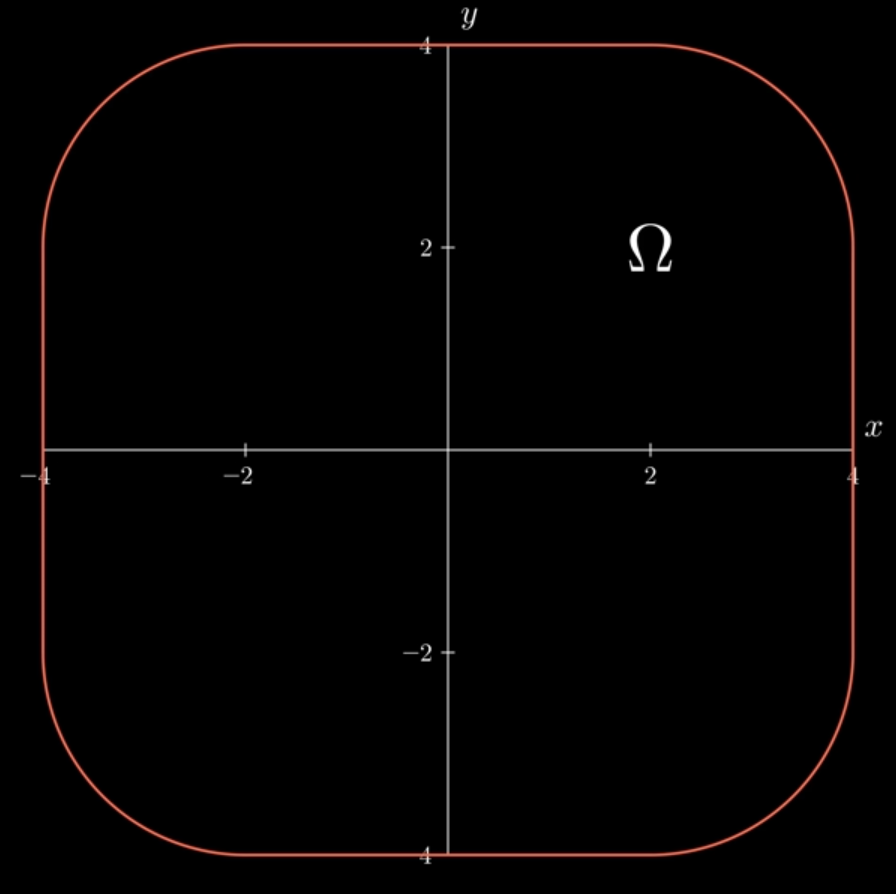
\includegraphics[height=8cm]{Region}
  + $\Omega$ % Idea: Had a circle in Q1 with \Omega in the center of the circle
\end{center}

Now, let us consider a point within this interval, $x_0$. Here, let us consider point $x_0$ to be an arbitrary point within our area, $\Omega$:

\begin{center}
  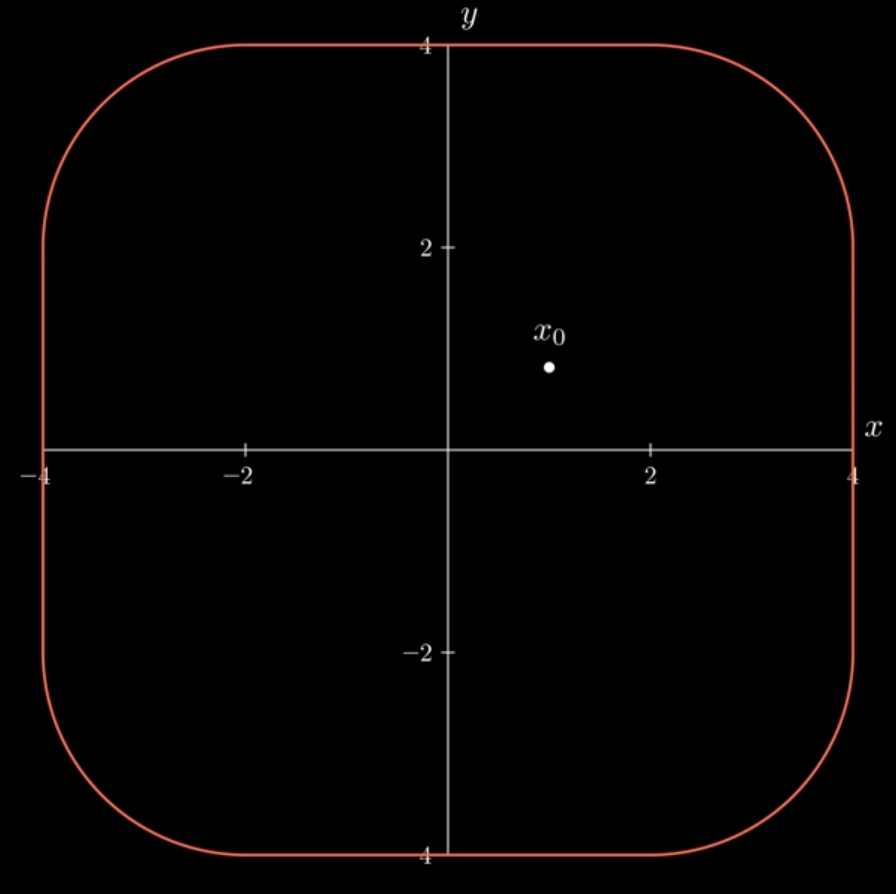
\includegraphics[height=8cm]{x0_0}
  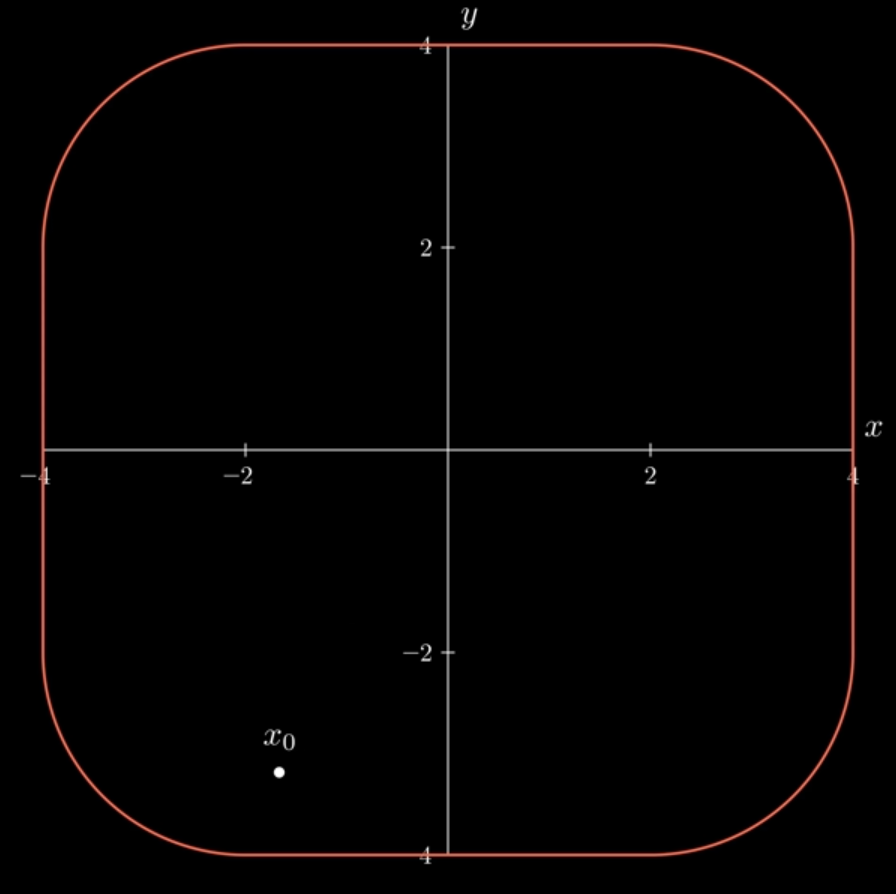
\includegraphics[height=8cm]{x0_1}
  % Move $x_0$ around \Omega
\end{center}

To begin, let us consider a neighborhood, or ball, around our point, $x_0$. Here, our ball around $x_0$, has a radius $\eps$, where $\eps > 0$, and the area of our ball is a subset of $\Omega$.

\begin{center}
  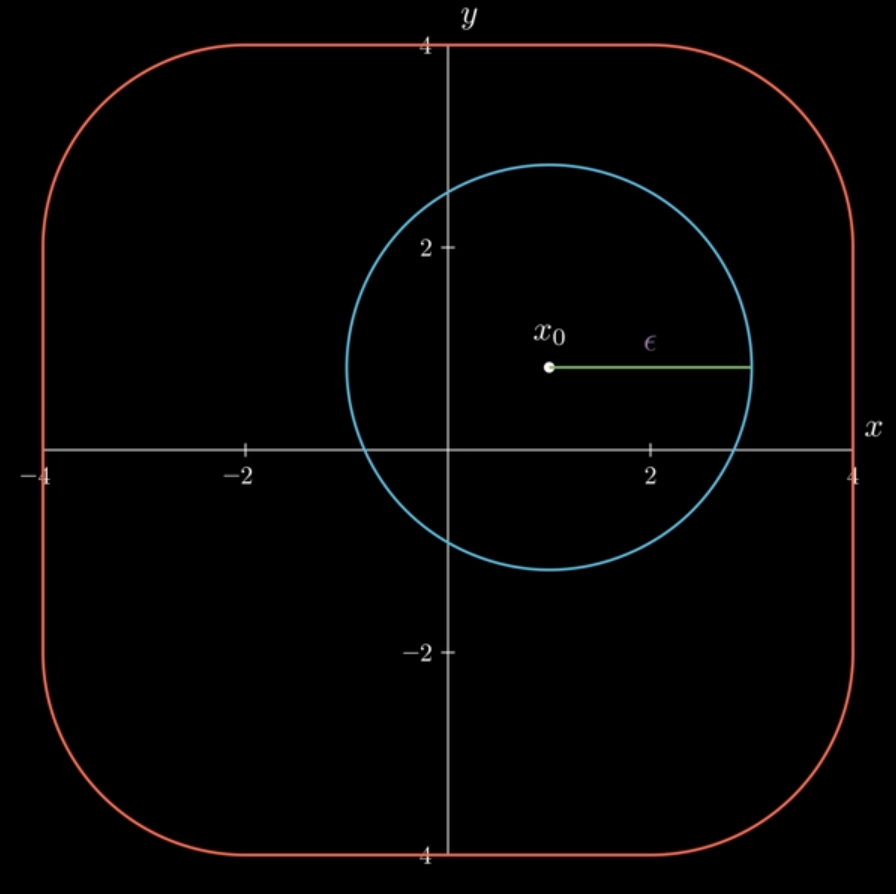
\includegraphics[height=8cm]{eps_0}
  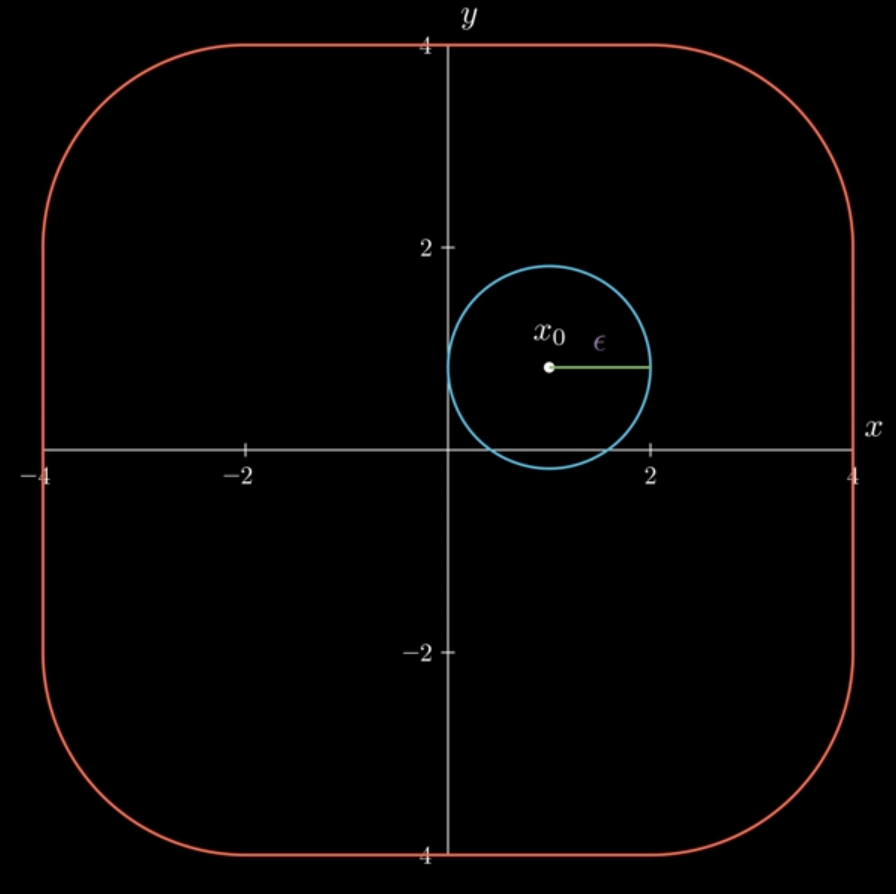
\includegraphics[height=8cm]{eps_1}
  % Static x_0 point, change the size of \eps, spanning from x_0 to \p \Omega
\end{center}

Now, let us consider what is $u(x)$. Here, $u(x)$ is a harmonic function,
allowing us to make the assumption that the average value of the function
within its neighborhood is the center point of our neighborhood. In this case,
our neighborhood is centered about $x_0$.

\begin{center}
  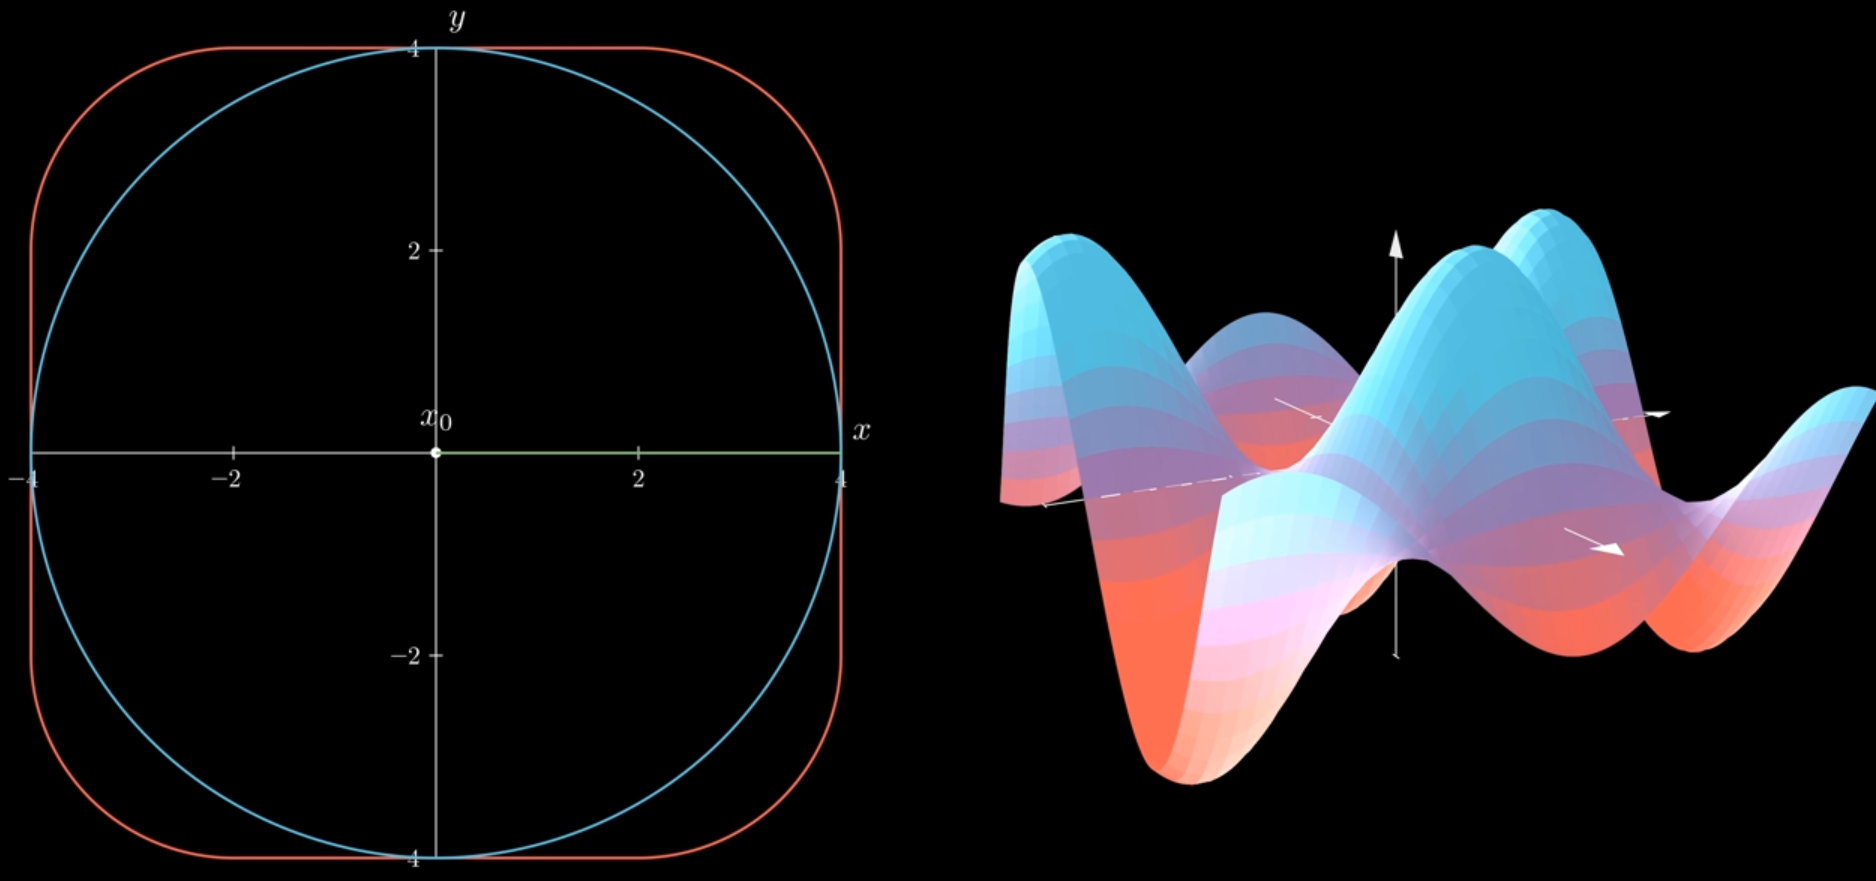
\includegraphics[height=8cm]{harmonic_base}
  % x_0 in the center, introduce a harmonic graph on the left and a 2-d graph
  % on the right with $x_0$ moving around along with $\eps$
\end{center}

Here, let us consider a function where the average value of its neighborhood
is also the maximum value of our harmonic function, $u(x)$. Here, if our
neighborhood's average value is always the maximum value throughout the
region, then our harmonic function's value is uniform throughout the region.
In other words, there is a constant value throughout the region.

\begin{center}
  % Constant harmonic function, move throughout the region
\end{center}

While the average of our neighborhood is considered the max in a constant function as shown, a function like this will not always occur.
% QUESTIONABLE CONTENT HERE
Here,
